\section{Trajectory Clustering}
\label{sec:trajCluster}

A similar problem to \trajSummary is clustering of generic trajectories, which has been studied for different purposes~\cite{Lee2007,Li2010}. We briefly describe and illustrate existing trajectory clustering mechanisms, and show that they do not provide good spatial summaries for trips of individuals. We then propose parametric and non-parametric techniques that utilize different distance metrics for effective clustering of user trips.

\subsection{Trajectory-distance Unaware Techniques}

\paragraph{TRACLUS}
TRACLUS is a frequently used algorithm for clustering trajectories. It is based on the \emph{partition-and-group} framework. TRACLUS relies on discovering similar  sub-trajectories, and doesn't look at them as a whole. In the first phase, the trajectories are partitioned into line segments based on Minimum Description Length principle. Once the trajectories are partitioned, it runs a density based clustering on the line segments based on two parameters, $\operatorname{minPts}$ and $\epsilon$. 
\\
We implemented TRACLUS, and used simulated annealing to arrive at the values of the parameters. TRACLUS was designed to detect animal movement, and trace hurricane patterns. In such cases, sub trajectory similarity played an important rule, which TRACLUS exploits. But in the case of human mobility or movement summarization, we want to look at entire end to end trips, and not delve into the sub-trajectory level. 

\begin{figure}
\begin{center}
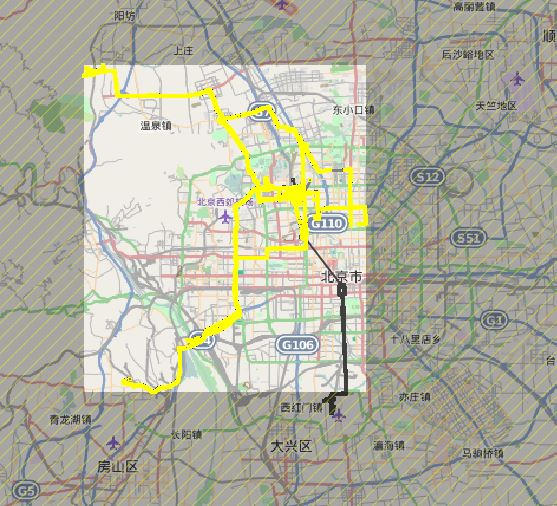
\includegraphics[width=3.5cm]{figs/TrajClus_cluster.jpg}
\end{center}
\caption{TRA-CLUS illustration: The large number of trajectories in a large area (in yellow color) are reported as primary cluster}
\label{fig:TrajClus_cluster}
\end{figure}

\paragraph{Swarm}
SWARM is a clustering method which clubs similarly moving objects together in a cluster. If a minimum $m_{0}$ number of individuals in a group fall in the same cluster for at-least a minimum number($min_{t}$) of non-consecutive timestamps, a swarm is reported. A swarm is a closed swarm if neither its Object set nor its Timestamp set can be further extended. The algorithms finds such closed swarms by doing a DFS on all the subsets of object timestamp pairs, with different rules to prune the search space.
To suit our problem, we considered the ordering of the points in the trajectory to be the timestamp value for that point. \\
To suit our problem, we considered the ordering of the points in the trajectory to be the timestamp value for that point. Making this assumption we took all the trajectories of the user to be the set of objects and identified closed swarms. As the points might not be sampled in a similar fashion, SWARM might miss out on similar clusters even though they are close to each other. 

\subsection{Trajectory-distance Aware Techniques}
\label{sec:trajDistClustAlgos}
Standard clustering approaches can be used with the trajectory distance measures mentioned in Section~\ref{sec:trajDist}. However, obtaining optimal clusters that describe meaningful user trip summaries require extensive analysis and experimentation of clustering approaches. We now describe the clustering algorithms and techniques to compute optimal user trip clusters.

\paragraph{DBSCAN}
\label{sec:dbscan}
Density-based spatial clustering of applications with noise (DBSCAN) is a widely used clustering algorithm which clusters closely connected points (dense neighborhoods)~\cite{ref:dbscan}. DBSCAN inputs two parameters: minimum number of neighborhood points ($\operatorname{minPts}$) and a neighborhood distance radius ($\epsilon$). 

Using the above parameters, DBSCAN categorizes each point as a core, reachable or outlier points. A core point is defined as a point which has at-least $\operatorname{minPts}$ within a radius of $\epsilon$. Reachable points are points which has less than $\operatorname{minPts}$ in its $\epsilon$-neighborhood, but there is at-least one core point within its $\epsilon$ distance. Rest of the points are termed as outliers. DBSCAN hence forms a cluster of core points with possible reachable points in the boundary. 

In our application, we show that DBSCAN is not the right clustering method irrespective of the distance metric used because of the fixed selection of neighborhood thresholds ($\operatorname{minPts}$ and $\epsilon$). This hinders the ability to find meaningful summaries in scenarios where users have, say, a mix of long and short trips. Here, we require the long distance trips to have a larger $\epsilon$ than for the shorter trips since such a property allows larger detours for long trips than for short trips. Note that parameter tuning will not yield meaningful summaries in the above cases since: (1) Increasing $\epsilon$ (or decreasing $\operatorname{minPts}$) will lead to clustering a large number of dissimilar smaller trips (small $\operatorname{minPts}$ or large $\epsilon$); or (2) Small values of $\epsilon$ may unnecessarily break similar long trips which have a slightly higher detour. Hence, our application requires clustering mechanism that accounts for selecting the distance thresholds which are based on the subset of neighboring trajectories. 

\begin{figure}
    \mbox{
				\begin{subfigure}[t]{.25\textwidth}
        \centering
        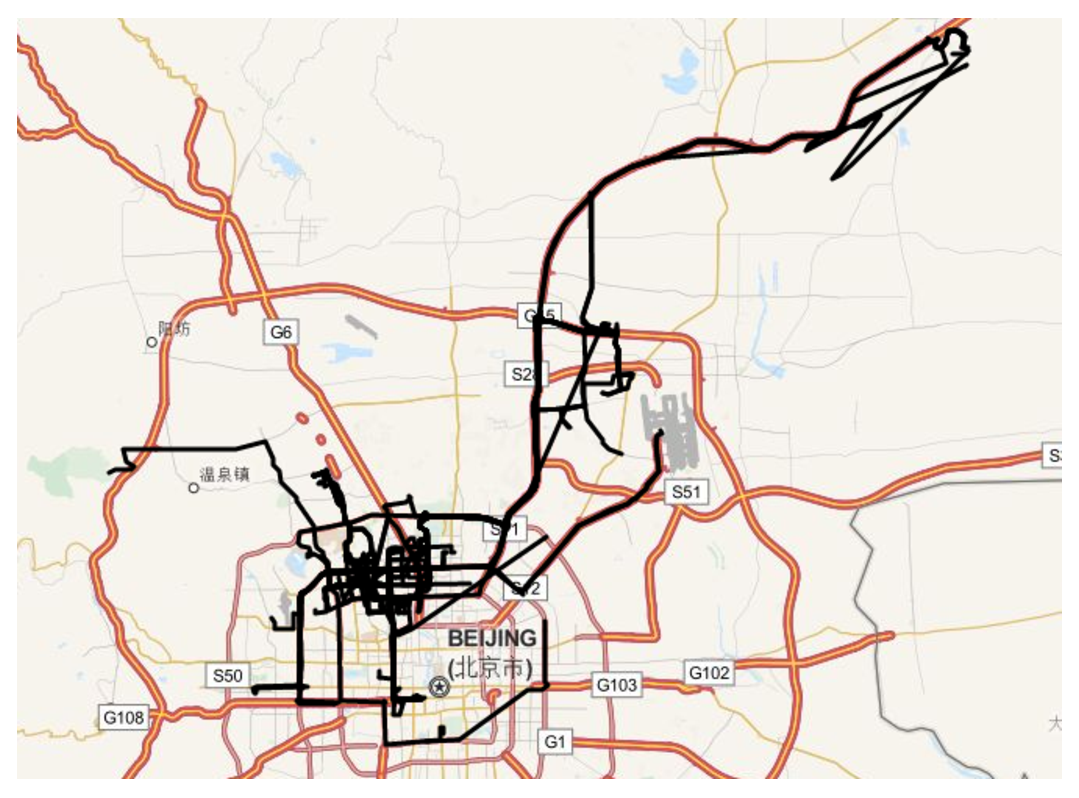
\includegraphics[height=3.6cm]{figs/new/allTrajs.eps}
        \caption{All trajectories of a user}
				\label{fig:allTrajs}
    \end{subfigure}%
		~
    \begin{subfigure}[t]{.15\textwidth}
        \centering
        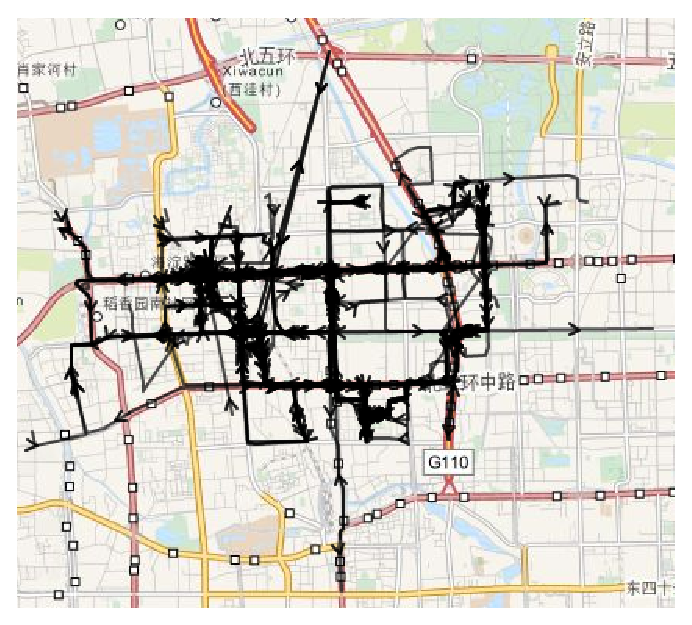
\includegraphics[width=4cm]{figs/dbscn_cluster1.eps}
        \caption{Cluster 1 (227 trajectories)}
    \end{subfigure}%
    }
		\mbox{
    \begin{subfigure}[t]{.2\textwidth}
        \centering
        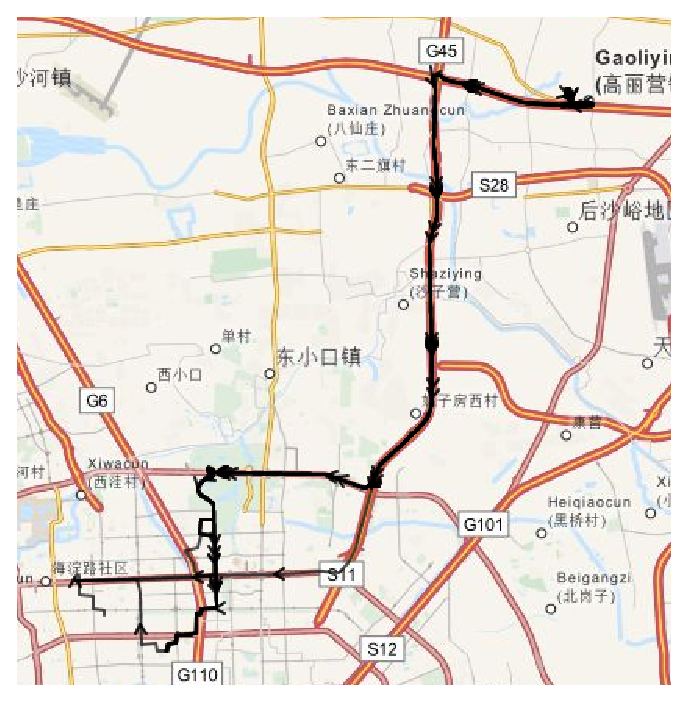
\includegraphics[height=4cm]{figs/dbscan_cluster2.eps}
        \caption{Cluster 2(4 trajectories)}
    \end{subfigure}
    ~
    \begin{subfigure}[t]{.2\textwidth}
        \centering
        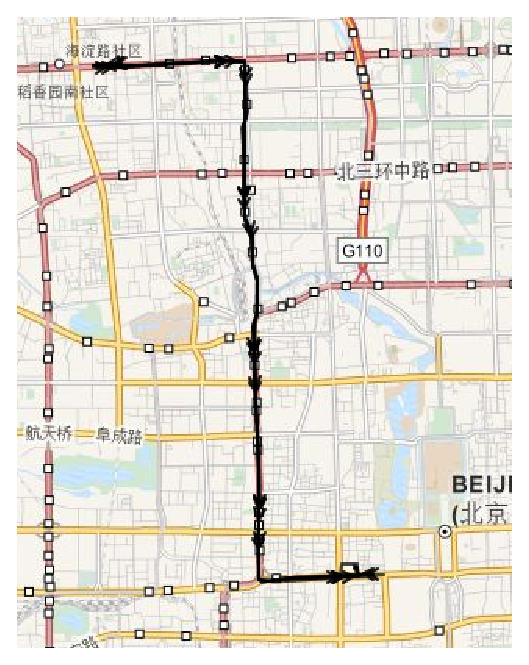
\includegraphics[height=4cm]{figs/dbscan_cluster3.eps}
        \caption{Cluster 3(4 trajectories)}
    \end{subfigure}%
    }
    \caption{Sample user and DBSCAN: Sample user with 323 trajectories. Top summary clusters in DBSCAN summarize user movement poorly}
    \label{fig:DBSCANRes}
\end{figure}
Figure~\ref{fig:DBSCANRes} shows a sample user with 323 trajectories, and the top-3 clusters detected by the DBSCAN with $\UN$ distance metric. We used the \textit{Sorted $k$-dist Graph} methodology proposed in DBSCAN~\cite{ref:dbscan} to compute the optimal values input parameters (which were $\operatorname{minPts}=5$ and $\epsilon=3$ in this scenario). The top cluster has 227 out of 323 trips, and is clearly not summarized user trips well. We tuned the parameters manually to check if we get better clusters. The configuration where $\epsilon=1$ provided better results, but the resulting clusters were not significantly different. 

\paragraph{Hierarchical Clustering}
Hierarchical agglomerative clustering is a bottom-up technique where the algorithm starts by considering each point as a cluster, and merges two `closest' clusters are aggregated to form a higher level cluster. This process is repeated until we reach a single cluster of all points. The definition of closeness of a cluster can be defined in many ways such as complete-linkage, single-linkage or average-link. Hence, Hierarchical clustering forms a tree (usually represented by a dendrogram) where a single cluster of points is repetitively split into two clusters until leaf nodes are reached~\cite{ref:hac}. 

Hierarchical clustering provides the flexibility of analyzing the entire history of user's trajectories, and then cutting the tree at the right level. This enables us to iterate down the tree, and estimate if the sub-tree forms a good cluster based on the distances between the trajectories and other parameters such as the trajectory lengths. We use complete-linkage measure define the distance between two intermediate clusters since it enables us to identify summaries where maximum distance between two trips in the summary is contained.

\subsection{Cluster Identification}
While standard distance metrics and clustering algorithms are well-known, choosing the right metric, clustering algorithm and the parameters for the application is a challenging task. Based on the requires for clustering user trips, we now discuss important approaches and techniques to identify superior summaries. 

Recall that $\UN$ metric is most suited to describe distance between user trips since it provides us an ability to measure the maximum detours between two trips (Section~\ref{sec:trajDist}). Similarly, we motivated the use of hierarchical clustering because of the ability to iterate down the tree, and examine if the trajectories under the tree are similar in terms of trajectory distances and other parameters such as trajectory lengths. 

\begin{figure}
    \mbox{
	 \begin{subfigure}[t]{.2\textwidth}
        \centering
        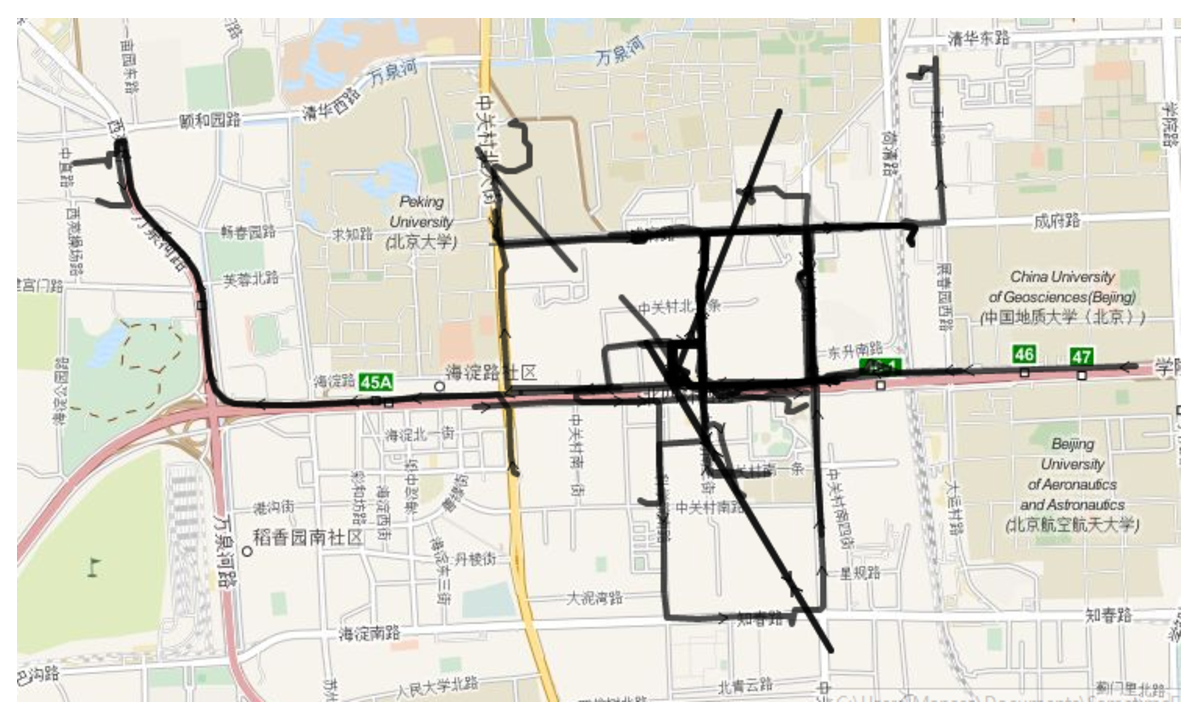
\includegraphics[width=4cm]{figs/new/Elbow_Cluster1.eps}
        \caption{Cluster 1 (32 trajectories)}
    \end{subfigure}%
		~
    \begin{subfigure}[t]{.2\textwidth}
        \centering
        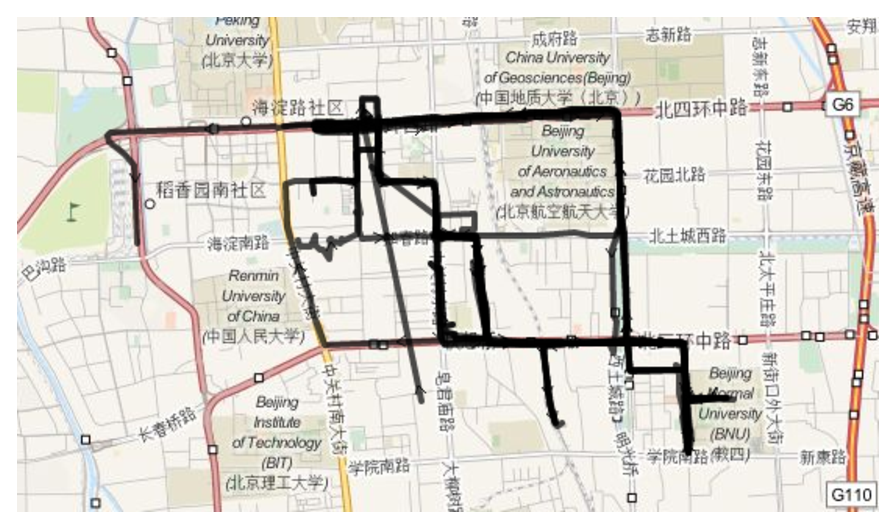
\includegraphics[width=4cm]{figs/new/Elbow_Cluster2.eps}
        \caption{Cluster 2 (31 trajectories)}
    \end{subfigure}
    }
		\mbox{
    \begin{subfigure}[t]{.2\textwidth}
        \centering
        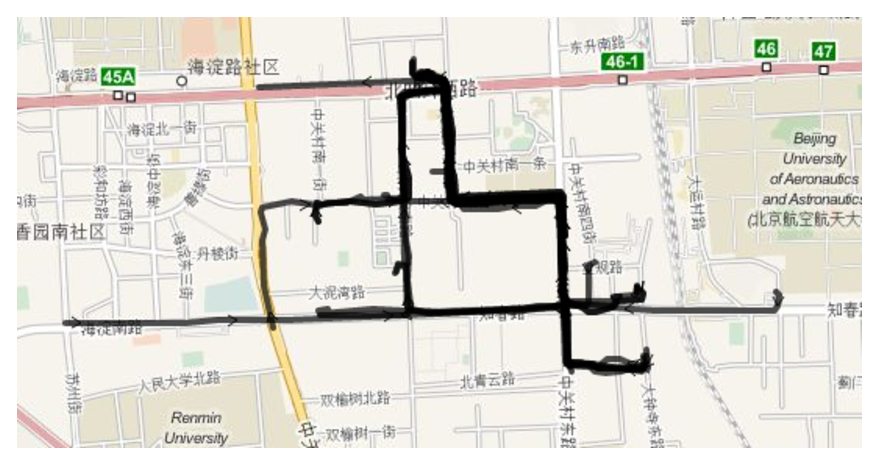
\includegraphics[width=4cm]{figs/new/Elbow_Cluster3.eps}
        \caption{Cluster 3 (31 trajectories)}
    \end{subfigure}%
		\begin{subfigure}[t]{.2\textwidth}
        \centering
        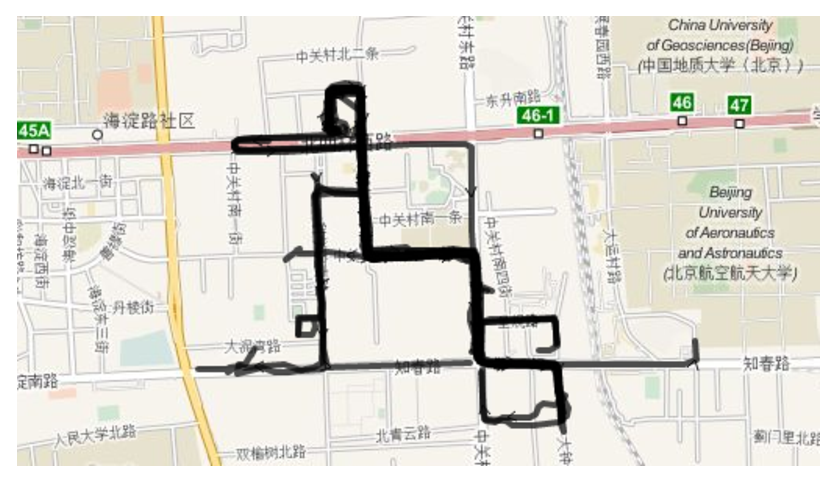
\includegraphics[width=4cm]{figs/new/Elbow_Cluster4.eps}
        \caption{Cluster 4 (31 trajectories)}
    \end{subfigure}
		}
    \caption{Elbow Method: Top-4 summary clusters detected are noisy and unusable}
    \label{fig:elbowVisual}
\end{figure}

Figure~\ref{fig:elbowVisual} shows top-4 clusters detected by the Elbow Method. Clearly, the summaries computed have a lot of dissimilar trips of the user since the elbow point stops at a very low value of $k$.

We first describe well-known Elbow Method to detect optimal number of clusters. Elbow method is widely used in literature to detect the optimal number of clusters for the data-set. Elbow method computes the cumulative \textit{Sum of Squared Errors} (SSE) within the cluster for increasing number of clusters (clusters $k=1,\ldots,N$ having $\operatorname{SSE}=\operatorname{SSE}_1,\ldots,\operatorname{SSE}_N$). SSE decreases as we increase the number of clusters. Elbow method picks the optimal number of clusters as the value of $k$ where the reduction of SSE becomes marginal when compared to reduction in the previous step

The elbow point is determined by plotting $k_i$ vs. $SSE_i$ and picking the $k_i$ which has the largest distance from the line drawn from $SSE_1$ to $SSE_k$. In hierarchical clustering, we can increase $k=1,\dots,N$ by iterating down the tree to find the elbow point.

Identifying the elbow point is non-obvious. We show in Section~\ref{sec:evalSumm} that, in most of the cases, choosing the elbow point results in far inferior summaries; the optimal clusters are far beyond elbow point in most cases. We now propose three new algorithms to identify superior user trip summaries.

\paragraph{\thresh}
\label{sec:thresh}
THRESH is a parametric heuristic to find reasonable clusters of trips. Here, we assume that the analyst can provide a threshold $T$ that signifies the maximum distance between any two trajectories in a cluster (say, \unit{1}{km}). We follow the below steps to identify the trip clusters:
\begin{enumerate}[label=S\arabic*:,topsep=0pt,itemsep=-1ex,partopsep=1ex,parsep=1ex]
\item Compute the distance matrix between trajectories using $\UN$
\item Iterate the dendrogram starting from the root using Breadth-First-Search (BFS).
\item At each node $i$, compute the maximum distance $\operatorname{maxDist}_i$ between all the trajectories under the node $i$. 
\item If the $\operatorname{maxDist}_i < T$, then mark all the trajectories under the node $i$ as a cluster, and delete the sub-tree from node $i$.
\item Else, visit the next node $i$ using BFS. Go to Step 3.
\end{enumerate}

Figure~\ref{fig:threshTopClusters} shows the summary clusters detected by \thresh for the user with trajectories shown in Figure~\ref{fig:allTrajs}. This is clearly superior than the clusters detected by the Elbow Method (Figure~\ref{fig:elbowVisual}) and DBSCAN (Figure~\ref{fig:DBSCANRes})

\begin{figure}
    \mbox{
    \begin{subfigure}[t]{.2\textwidth}
        \centering
        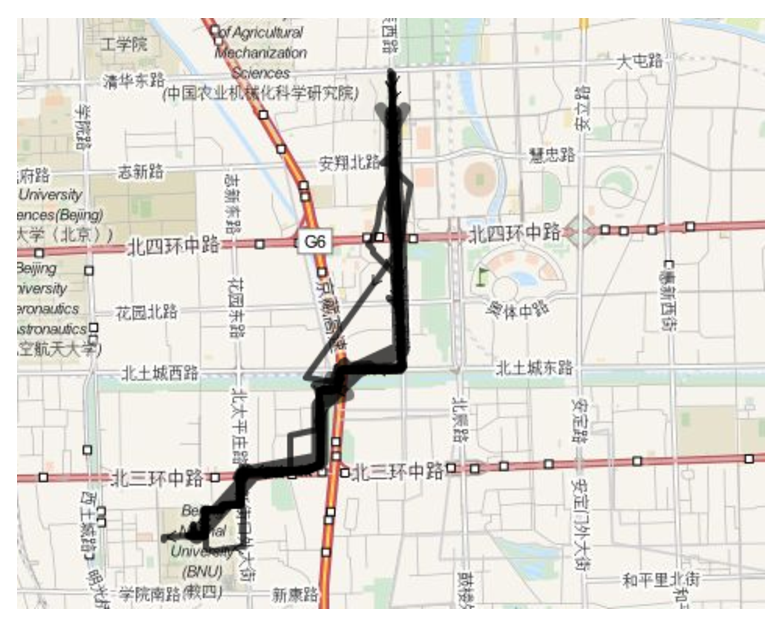
\includegraphics[width=4cm]{figs/new/FinalCluster1.eps}
        \caption{Cluster 1 (20 trajectories)}
    \end{subfigure}%
     
    \begin{subfigure}[t]{.2\textwidth}
        \centering
        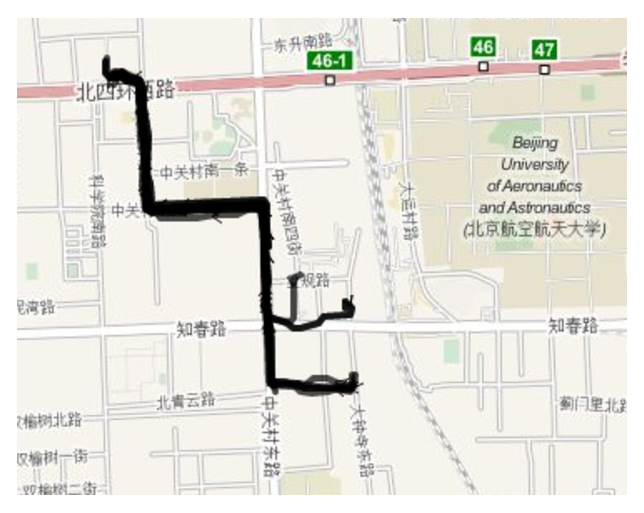
\includegraphics[width=4cm]{figs/new/FinalCluster2.eps}
        \caption{Cluster 2 (15 trajectories)}
    \end{subfigure}
    }
		\mbox{
    \begin{subfigure}[t]{.2\textwidth}
        \centering
        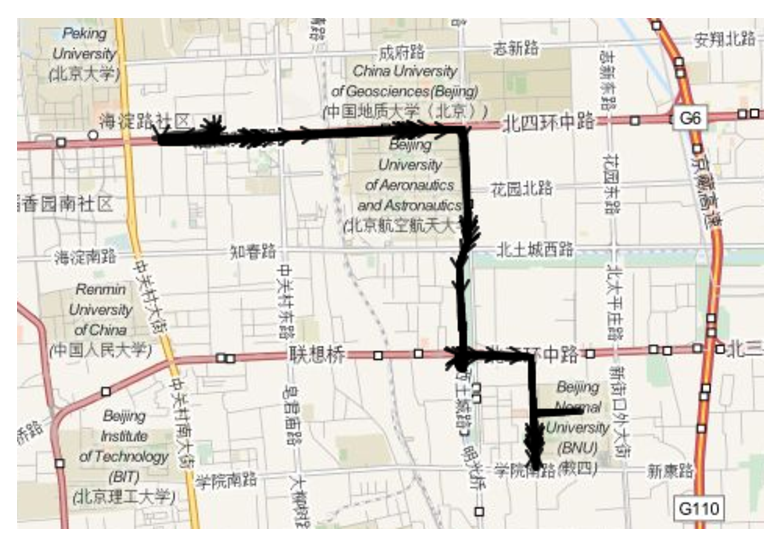
\includegraphics[width=4cm]{figs/new/FinalCluster3.eps}
        \caption{Cluster 3(11 trajectories)}
    \end{subfigure}%
    \begin{subfigure}[t]{.2\textwidth}
        \centering
        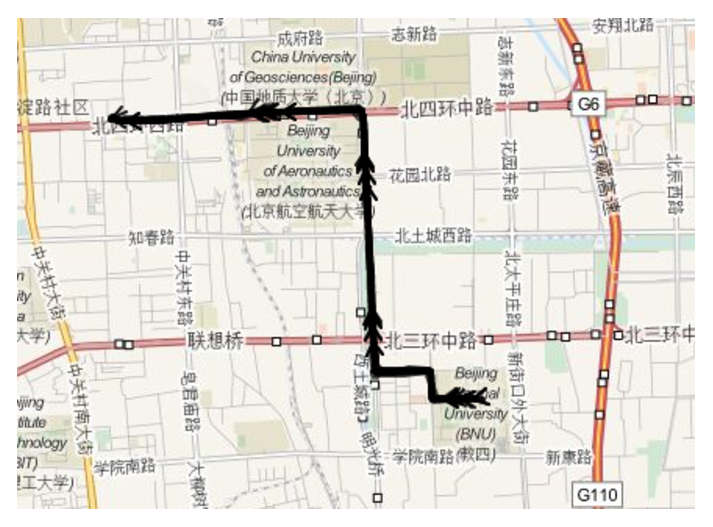
\includegraphics[width=4cm]{figs/new/FinalCluster4.eps}
        \caption{Cluster 4(9 trajectories)}
    \end{subfigure}
		}
    \caption{\thresh: Top-4 summary clusters}
    \label{fig:threshTopClusters}
\end{figure}

\paragraph{\lthAware}
\begin{comment}
\begin{figure}[t!]
\centering
 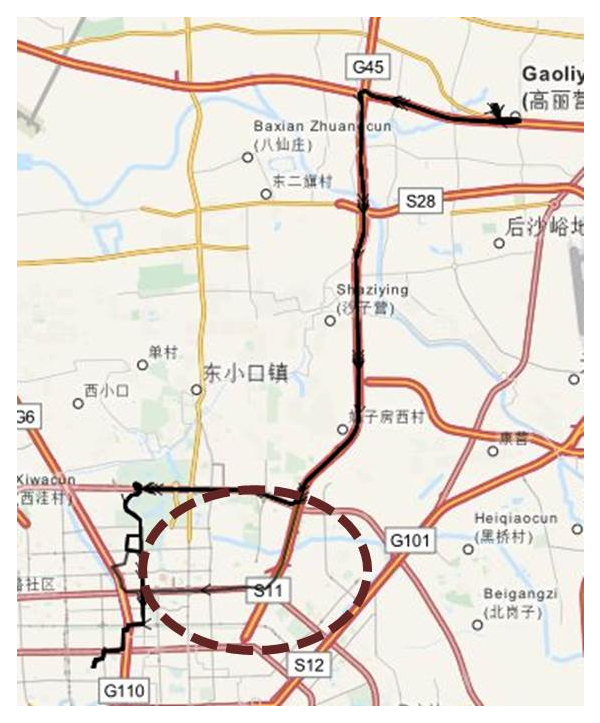
\includegraphics[width=12cm,height=3cm,keepaspectratio]{figs/longtrajs.eps}
 \caption{A cluster with a detour in the middle -- Cluster reported by Modal analysis}
 \label{fig:modal}
 \end{figure}
\end{comment}

Consider a user whose regularly commutes from home to two offices: an office \unit{100}{km} from home and another \unit{5}{km}. Clearly, a deviation of $\unit{1}{km}$ is tolerable while considering the \unit{100}{km} trajectories, and not in the \unit{5}{km} commute trip from home to work. \thresh will be unable to separate these two clusters since it is non-cognizant of the trajectory lengths. We propose a trajectory length aware algorithm \lthAware to overcome this problem. \lthAware operates similar to \thresh algorithm (Section~\ref{sec:thresh}). However, at each node $i$, it computes the trajectory length normalized standardized deviation ($\operatorname{nsd_i}$) as
\begin{align}
	\operatorname{nsd_i}=\frac{\text{std dev of distances between trajectory-pairs under node }i}{\text{mean trajectory length of all trips under node }i}.
\end{align}

The analyst provides a value of tolerable fraction threshold $\operatorname{NSD}$ (say, 0.1 in our case). Steps S4 in \thresh is then changed to the below:
\begin{enumerate}[label=S\arabic*:]
\setcounter{enumi}{4}
\item If the $\operatorname{nsd}_i < \operatorname{NSD}$, then mark all the trajectories under the node $i$ as a cluster, and delete the sub-tree from node $i$.
\end{enumerate}

In Section~\ref{sec:evalSumm}, we show that \lthAware provides a clean separation of trips for users who have regular inter- and intra-city commutes. 

\paragraph{\modal}
\begin{figure*}
\centering
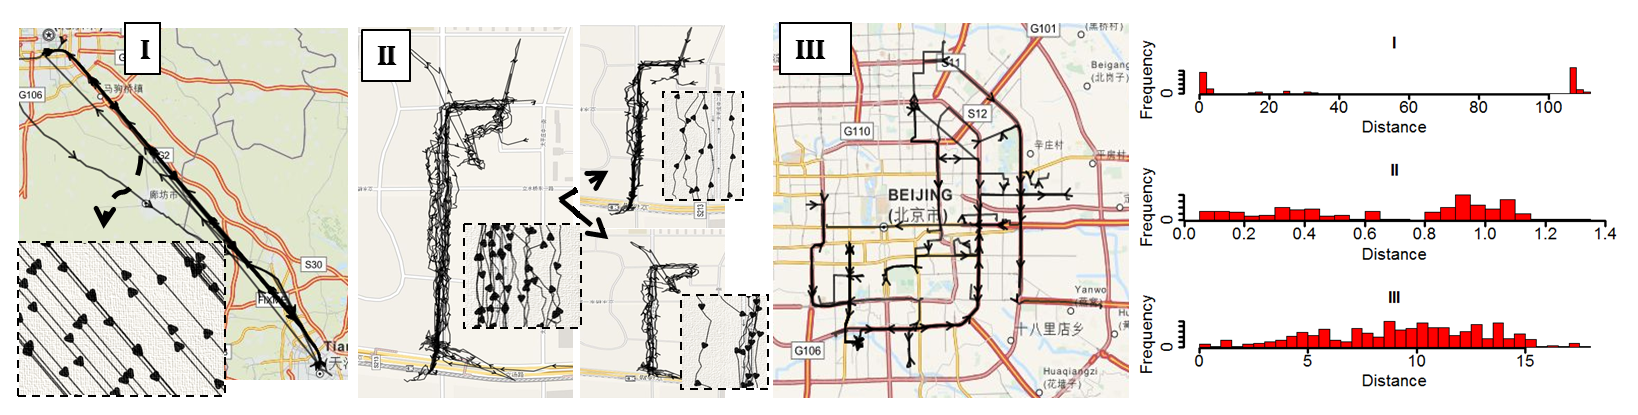
\includegraphics[scale=0.6]{figs/hist_full.eps}
\caption{Illustration of non-parametric nature of MODE-EST: Figs. I and II show the long and short trips. Fig. III shows anomalous cluster. Fig IV shows the bi-modal distribution for Figs. I and II, and unimodal distribution with large mean for Fig. III}
\label{fig:anom}
\end{figure*}

While \lthAware allows trajectory clustering based on the length of the trajectories, it still requires an input parameter that is tuned. We now propose a non-parametric technique that estimates effective clusters without any fixed thresholds. As stated above, standard non-parametric estimates such as Elbow Method do not directly provide good clusters. Hence, we design a technique that examines the distribution of the distances and, based on the number of modes, decides to proceed consider the sub-tree at node $i$ as a cluster or iterate down the tree.

Note that if there are large number of similar trips under a sub-tree at node $i$, then the distance between such trips will be constant, and will appear as a significant mode in the probability density function. We implement the non-parametric test of number of modes using the approach described by Minnotte \textit{et. al.}~\cite{minnotte}. We find the number of modes in the kernel density plot of the pair-wise trajectory distances under node $i$. If there is a single mode, then we accept it as a  cluster of similar trajectories. Else we iterate down the tree. 

However, there is another interesting possibility. The distance distribution under node $i$ might have a single mode, but the distances may be spread out over a very large range. Such a distribution indicates that the trips under node $i$ most probably does not contain any cluster of similar trips; a set of anomalous trips have such characteristics. Hence, we add a post-processing stage to check the condition of anomalous cluster: if there is a single mode and the mean of pair-wise trajectory distances is greater than some large distance $L$. If such anomalous cluster condition is detected, then we prune out the node $i$ without accepting the underlying trajectories as a cluster of similar trajectories. This also saves computation time since we do not iterate down the sub-tree.

We now illustrate the modes and the distance distribution in our dataset. Figure~\ref{fig:anom} (I and II) shows the bi-modal distribution of long inter-city trajectories between Beijing and Tianjin (\unit{135}{km}) and short intra-city (\unit{1}{km}) trips, where the to- and fro-trips have different distances between each other. Figure \ref{fig:anom} III shows an anomalous cluster detected with the corresponding histogram of distances.

% Final summary
In all the above schemes, we finally represent the ``Summary Clusters'' of a user as the clusters with number of trajectories greater than a certain threshold (5\% of user's trajectories in our case)

\begin{comment}
\subsection{Finding optimal clusters}
Number of clusters in the summary: Since each person's movement is unique(?), the number of clusters and the number of trajectories expected in each clusters are not constant. Hence, standard mechanisms such as k-means clustering cannot be directly applied to summarize. Even after the clusters are found out, we need to see if this cluster represents points that have meaningful end-to-end trips.% \rednote{This is not coming out good. Need to think}
We need good OD +  we need trajectories that are not far away in the middle. One way to design a sim metric that is cognizant of: (1) origins, destinations, directionality and (2) the maximum separation between the trajectories. However, such a sim metric will introduce other artifacts (say, by classifying far away trajectories into same cluster). Hence we consider an approach where we decouple by considering O/D and direction in the sim metric, and then design an algorithm to select optimal number of clusters by looking at the maximum intra-cluster separation.
\end{comment}

\subsection{Representative trajectories}
\label{sec:repTraj}
We now find a representative trajectory for each of the cluster that can be used as a proxy for a Summary Cluster. One approach is to consider the mean trajectory curve $\meanTraj_i$ as a representative for the cluster $\summClus_i$. However, since the mean of multiple curves may not fall on any of the individual trajectories (and hence the roads on which the user went), it is not recommended as a representative. Hence, we follow a well-known method of computing piece-wise median trajectories~\cite{median1}. Here, at an interval of $\delta$ number of points on interpolated mean trajectory, one point on any of the trajectories in the cluster closest to the mean is added to the representative trajectory. 

\begin{comment}
\subsection{Storing the trajectories at various levels of granularity}
\subsection{Intra-cluster Movement Pattern}
\end{comment}

\begin{comment}
Similarity metric for summarizing human movement should consider the below aspects
\begin{itemize}
\item Importance to Origins and Destinations: Hurricanes and other physical effects (?) are generally governed by physical laws and computing similarity might have to account for different effects. However, movement of a people is generally associated with an intention (such as commuting to work) of moving from an origin point to a destination point. Hence, a reasonable summary of a person's movement accounts for end-to-end trips that she takes. Currently, there is no similarity metric that gives any bias to the endpoints of the trajectory. We try to plug the bias into our similarity metric so that trip intentions are also given importance. 
For example, SWARM does not consider explicitly consider the end points of the trajectory. Hence, it might wrongly categorize movement on similar roads -- even with varying end points -- into the same cluster. %\rednote{Show a toy scenario that shows how SWARM has mistook two different o-d clusters to be in the same cluster}

\item Metric: Clustering trajectories using standard clustering algorithms require the distance function between two trajectories to be a mathematical metric. In the current literature, only a few functions are metrics \cite{lp,edwp}. Others, which mostly take care of artifacts of sampling, are shown to be non-metrics. Using such functions, which violate properties like triangular inequality, in clustering can lead to unforeseen results. %\rednote{Show a figure where tri inequality is violated in actual sense}
Ex of triangle inequality - User 014 ; Trajs 3,11,175;
3-175(124)>3-11(94)+11-175(4.283)

\item Sampling artifacts: Is time stretching and shrinking important? Are sampling points important? Ours is better because we consider human specific movement where direction and OD are important. While sampling frequency and alignment of samples is required, more or less all traces can be preprocessed after good samples have been taken. So, it really doesnt make sense to consider the effect of timing of samples (like DTW) while designing the clustering algorithm. %\rednote{Vinay: Show a toy scenario where DTW goes wrong}
\end{itemize}

\paragraph{Origin-Destination}
In human movement, similar trips are usually between similar origin and destination regions. For example, the summary of a vast majority of working population are their trajectories between home and office. Hence, the similarity function should provide greater importance to OD. We define \textit{Weighted LP-Norm for OD} as
\begin{align}
w_{\od}(t, c, r) &= 
	\begin{cases} 
		\frac{c}{r} &\mbox{if } t \le \frac{r}{2} \mbox{ or } t > (1 - \frac{r}{2}), \\ 
		\frac{1- \frac{c}{r}}{(1-r)} & \mbox{otherwise},
	\end{cases}
\end{align}
\noindent where $r$ and $c$ denote the parameters define the weight assigned to the origin and destination stretches when compared to the intermediate stretch. Here $r$ defines the fraction of the stretch from origin or towards destination which has to be given a prominence ($r=[0,1]$). And, $c$ is the weight assignment factor at O and D stretches ($c=[0,1]$). If $c > 1 -r$, then the origin and destination stretches of length $\frac{r}{2}$, will be given a higher weight than the intermediate stretch (of length $1 - r$)


\noindent
For Uma's work:
Let $x_i \ge 0$ represent the ``color of grid $i$''. \\
Let $N(i) = \left \{ \text{All grids that are neighbors of i} \right \}$. \\
Let $C$ be the ``conflicting set''. A tuple $(i,j)$ is added to the conflicting set $C$ if two grids $i$ and $j$ have a \textit{LAC separating line} between them.\\
Let $y_i$ be an indicator variable to say if the grid has same color as at-least one of its neighbor.

We formulate an optimization problem to find the color for each grid as below:
\begin{align}
\mbox{Min} \sum_{i}{y_i}
\end{align}
\noindent such that:
\begin{align}
x_i &\neq x_j, ~~~\forall (i,j) \in C\\
y_i &= 
\begin{cases} 
		1 &\mbox{if } \forall j=N(i), x_i = x_j, \\ 
		0 &\mbox{otherwise}.
	\end{cases}
\end{align}

In order to assign similarity scores  to pairs of trajectories, we first have to resample them into equal number of points. 
\paragraph{Resampling and Interpolation}
\paragraph{Using Linear Interpolation over Spline}
%\rednote Image showing problems when using spline interpolation 
\begin{figure}
\centering
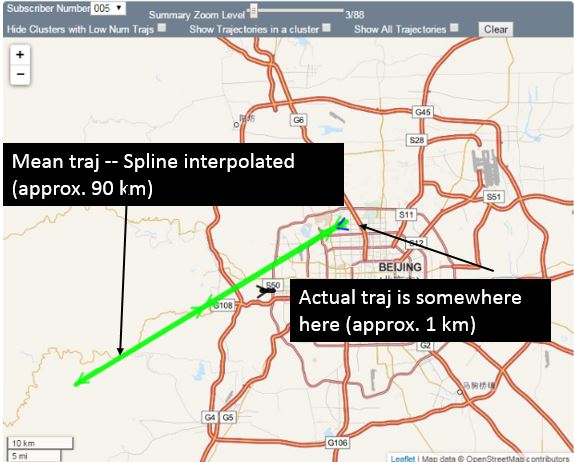
\includegraphics[scale=0.4]{figs/spline.jpg}
\caption{Problems with spline interpolation}
\label{fig:spline}
\end{figure}
\paragraph{Resampling and then applying DTW is very close to using our similarity measure }
\end{comment}